% =====================================================================
%  Phase 3 Report -- Acrobot (single column, one-and-a-half spacing)
%  Sections I-V: Phase 1 (model); Sections VI-IX: Phase 2 (stability)
% =====================================================================
\documentclass[10pt,letterpaper]{article}
\usepackage[top=0.5in,bottom=0.55in,left=0.7in,right=0.7in]{geometry}
\usepackage[T1]{fontenc}
\usepackage{mathptmx}\usepackage{amssymb}\renewcommand{\ttdefault}{pcr}
\usepackage{amsmath,graphicx,booktabs,array,microtype,xcolor,float}
\usepackage[compact]{titlesec}
\usepackage[labelsep=period,font=footnotesize]{caption}
\usepackage{enumitem}
\usepackage{cite}
\usepackage{xurl}
\usepackage{setspace}\onehalfspacing
\usepackage[hidelinks]{hyperref}

\renewcommand{\thesection}{\Roman{section}}
\renewcommand{\thesubsection}{\Alph{subsection}}
\titleformat{\section}{\normalfont\normalsize\scshape\bfseries}{\thesection.}{0.5em}{}
\titlespacing*{\section}{0pt}{5pt plus 2pt minus 1pt}{1pt plus 1pt}
\titleformat{\subsection}[runin]{\normalfont\normalsize\itshape\bfseries}{\thesubsection.}{0.4em}{}[.]
\titlespacing*{\subsection}{0pt}{3pt plus 1pt minus 1pt}{0.6em}
\renewcommand{\thetable}{\Roman{table}}
\captionsetup[figure]{name=Fig.,skip=2pt}
\captionsetup[table]{name=Table,labelfont=bf,skip=2pt}
\setlength{\parindent}{0pt}
\setlength{\parskip}{0pt}
\setlength{\abovedisplayskip}{2pt plus 1pt minus 1pt}
\setlength{\belowdisplayskip}{2pt plus 1pt minus 1pt}
\setlength{\abovedisplayshortskip}{0pt}
\setlength{\belowdisplayshortskip}{1pt}
\setlength{\intextsep}{3pt plus 1pt minus 2pt}
\setlist{leftmargin=1.1em,itemsep=0pt,topsep=1pt,parsep=0pt}
\setlength{\emergencystretch}{1.5em}
\allowdisplaybreaks\clubpenalty=0\widowpenalty=0\displaywidowpenalty=0
\newcommand{\Nm}{\,\mathrm{N\,m}}
\hyphenpenalty=10000\exhyphenpenalty=10000
\pagestyle{plain}
% a block that never splits across pages (moves whole to the next page)
\newenvironment{keep}{\par\noindent\begin{minipage}{\linewidth}}{\end{minipage}\par\smallskip}

\begin{document}

\begin{center}
\begin{singlespace}
{\fontsize{17}{20}\selectfont Phase 1: Modelling, Equilibria and Linearization of the Acrobot}\\[4pt]
{\small Bhargav (2025102061) \quad Sreekar (2025102074) \quad Kaushik (2025102071) \quad Divijat (2025102040)}\\[1pt]
{\footnotesize Control Systems Project \quad$\cdot$\quad Phase 1 Report \quad$\cdot$\quad October 25, 2026}
\end{singlespace}
\end{center}
\vspace{-6pt}
{\small\textbf{Abstract.} We verify the given Acrobot model, find its zero-torque equilibria, linearize at each, and derive the transfer functions from the elbow torque $\tau$ to both joint angles. Phase~2 (stability analysis) starts on page~\pageref{phase2} and Phase~3 (control) on page~\pageref{phase3}.\par}

% =====================================================================
\section{Nonlinear Model}
% =====================================================================
\noindent\begin{minipage}[t]{0.6\textwidth}\vspace{0pt}
\subsection{System and Parameters}
Two-link pendulum (Fig.~\ref{fig:schematic}) with a passive shoulder and a motor at the elbow [1], [2].
\begin{itemize}
\item Angles: $q_1$ = link~1 from the downward vertical; $q_2$ = link~2 relative to link~1; $\varphi=q_1+q_2$.
\item State: $x=[q_1,\;q_2,\;\dot q_1,\;\dot q_2]^T$.
\item Input: elbow motor torque $\tau$, $|\tau|\le20\Nm$, the only quantity we command ($\tau=0$ in this phase; set by a controller in later phases).
\item $m_1=m_2=1$~kg, $l_1=1$~m, $l_2=2$~m, $l_{c1}=0.5$~m, $l_{c2}=1$~m, $I_1=0.083$, $I_2=0.33$~kg\,m$^2$, $g=9.81$~m/s$^2$.
\end{itemize}
\subsection{Given Equations of Motion}
\begin{equation}
M(q)\ddot q+C(q,\dot q)\dot q=\tau_g(q)+B\tau,\qquad B=[0,\;1]^T\label{eq:eom}
\end{equation}
($B$ applies $\tau$ to the elbow equation only; $c_2=\cos q_2$, $s_2=\sin q_2$.)
\end{minipage}\hfill
\begin{minipage}[t]{0.36\textwidth}\vspace{0pt}
\centering
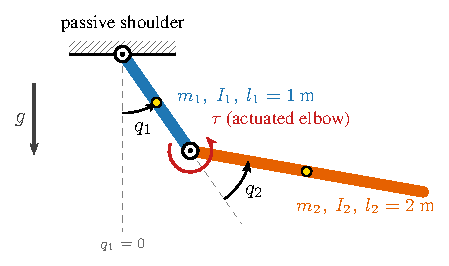
\includegraphics[width=\linewidth]{acrobot_diagram.pdf}
\captionof{figure}{Acrobot schematic (to scale); dots mark the centres of mass.}\label{fig:schematic}
\end{minipage}

\subsection{Derivation}
\textit{1) Potential energy and gravity torque:}
\begin{equation}
U=-(m_1l_{c1}+m_2l_1)g\cos q_1-m_2l_{c2}g\cos\varphi=-14.715\cos q_1-9.81\cos\varphi,\qquad
\tau_g=-\frac{\partial U}{\partial q}=-9.81\begin{bmatrix}1.5\sin q_1+\sin\varphi\\ \sin\varphi\end{bmatrix}.\label{eq:tg}
\end{equation}
\textit{2) Kinetic energy and inertia matrix:} the velocity of centre~2 is the elbow velocity ($l_1\dot q_1$) plus the rotation about the elbow ($l_{c2}\dot\varphi$), at angle $q_2$ apart (law of cosines):
\begin{equation}
T=\tfrac12(m_1l_{c1}^2+I_1)\dot q_1^2+\tfrac12I_2\dot\varphi^2+\tfrac12m_2\big(l_1^2\dot q_1^2+l_{c2}^2\dot\varphi^2+2l_1l_{c2}c_2\dot q_1\dot\varphi\big)=\tfrac12\dot q^TM\dot q,\quad
M(q)=\begin{bmatrix}2.663+2c_2 & 1.33+c_2\\ 1.33+c_2 & 1.33\end{bmatrix}.\label{eq:M}
\end{equation}
\textit{3) Coriolis term (Euler--Lagrange):} with $\partial T/\partial\dot q=M\dot q$ and $\dot M=\frac{\partial M}{\partial q_2}\dot q_2=-s_2\dot q_2\left[\begin{smallmatrix}2&1\\1&0\end{smallmatrix}\right]$,
\begin{equation}
\frac{d}{dt}\frac{\partial T}{\partial\dot q}-\frac{\partial T}{\partial q}=\tau_g+B\tau
\;\Rightarrow\; M\ddot q+\underbrace{\Big(\dot M\dot q-\frac{\partial T}{\partial q}\Big)}_{=\,C\dot q}=\tau_g+B\tau,
\qquad C(q,\dot q)=s_2\begin{bmatrix}-2\dot q_2 & -\dot q_2\\ \dot q_1 & 0\end{bmatrix}.\label{eq:C}
\end{equation}
These are the same $\tau_g$, $M$ and $C$ as in the given model.
\subsection{State-Space Form}
$M$ is always invertible, so solving~\eqref{eq:eom} for $\ddot q$ gives the state equation:
\begin{equation}
\det M=(2.663+2c_2)(1.33)-(1.33+c_2)^2=1.7729-c_2^2\ge0.7729>0\;\;(c_2^2\le1),\qquad
\dot x=f(x,\tau)=\begin{bmatrix}\dot q\\ M^{-1}\big(\tau_g+B\tau-C\dot q\big)\end{bmatrix}.\label{eq:f}
\end{equation}

% =====================================================================
\section{Equilibria}
% =====================================================================
\subsection{Conditions}
At rest $\dot q=\ddot q=0$, and the input torque is given as $\tau^*=0$. Then~\eqref{eq:eom} gives $\tau_g(q^*)=0$:
\begin{equation*}
\text{row 2: }\sin(q_1^*+q_2^*)=0,\qquad
\text{row 1: }1.5\sin q_1^*+\underbrace{\sin(q_1^*+q_2^*)}_{=0}=0\;\Rightarrow\;\sin q_1^*=0 .
\end{equation*}
\subsection{Solutions}
$q_1^*\in\{0,\pi\}$, $q_1^*+q_2^*\in\{0,\pi\}$ $\Rightarrow$ $q_2^*\in\{0,\pi\}$ (mod $2\pi$): \textbf{four equilibria}, all with both links vertical (Table~\ref{tab:eq}).

\begin{table}[h]
\centering
\caption{Equilibria for $\tau^*=0$}\label{tab:eq}
\footnotesize\setlength{\tabcolsep}{6pt}\renewcommand{\arraystretch}{0.9}
\begin{tabular}{@{}clcrl@{}}
\toprule
 & Posture & $(q_1^*,q_2^*)$ & $U$ [J] & Description\\
\midrule
$E_1$ & down--down & $(0,0)$ & $-24.525$ & both links hanging\\
$E_2$ & down--up & $(0,\pi)$ & $-4.905$ & link 1 down, link 2 up\\
$E_3$ & up--up & $(\pi,0)$ & $+24.525$ & fully upright (target)\\
$E_4$ & up--down & $(\pi,\pi)$ & $+4.905$ & link 1 up, link 2 down\\
\bottomrule
\end{tabular}
\end{table}

% =====================================================================
\section{Linearization}
% =====================================================================
\subsection{Deviation Variables}
$\tilde q=[q_1-q_1^*,\;q_2-q_2^*]^T$, $\tilde x=[\tilde q;\dot{\tilde q}]=x-x^*$, $\tilde\tau=\tau-\tau^*=\tau$. First-order Taylor expansion of~\eqref{eq:f} about $(x^*,0)$, using $f(x^*,0)=0$: $\dot{\tilde x}\approx\frac{\partial f}{\partial x}\big|_*\tilde x+\frac{\partial f}{\partial\tau}\big|_*\tilde\tau$.
\subsection{Jacobians}
\textit{Top half:} $\tfrac{d}{dt}\tilde q=\dot{\tilde q}$ $\Rightarrow$ rows $[\,0\;\;I_2\,]$. \textit{Bottom half:} $h=M^{-1}(\tau_g+B\tau-C\dot q)$; at $(x^*,0)$, $\partial(C\dot q)/\partial\dot q=0$ ($C\dot q$ is quadratic in $\dot q$, $\dot q^*=0$) and $(\partial M^{-1}/\partial q)(\tau_g+B\tau)=0$ ($\tau_g(q^*)=0$, $\tau^*=0$). Hence
\begin{equation}
\ddot{\tilde q}=P\tilde q+r\tilde\tau,\quad P=M(q^*)^{-1}K(q^*),\quad r=M(q^*)^{-1}B,\qquad
K(q^*)=\frac{\partial\tau_g}{\partial q}\Big|_{q^*}=-9.81\begin{bmatrix}1.5\cos q_1^*+\cos\varphi^* & \cos\varphi^*\\ \cos\varphi^* & \cos\varphi^*\end{bmatrix}.\label{eq:K}
\end{equation}
\subsection{Linear State-Space Model}
Stacking both halves, with the joint angles as outputs, $y=\tilde q=[q_1-q_1^*,\;q_2-q_2^*]^T$:
\begin{equation}
\boxed{\;\dot{\tilde x}=A\tilde x+B_\ell\tilde\tau,\quad y=C_y\tilde x+D\tilde\tau,\qquad
A=\begin{bmatrix}0 & I_2\\ P & 0\end{bmatrix}\!,\;
B_\ell=\begin{bmatrix}0\\ r\end{bmatrix}\!,\;
C_y=\begin{bmatrix}I_2 & 0\end{bmatrix}\!,\; D=0\;}\label{eq:AB}
\end{equation}
\subsection{Example: $E_1=(0,0)$} $\cos q_1^*=\cos\varphi^*=c_2=1$:
\begin{gather*}
K=\begin{bmatrix}-24.525&-9.81\\-9.81&-9.81\end{bmatrix}\!,\quad
M=\begin{bmatrix}4.663&2.33\\2.33&1.33\end{bmatrix}\!,\quad
\det M=0.7729,\quad M^{-1}=\frac{1}{0.7729}\begin{bmatrix}1.33&-2.33\\-2.33&4.663\end{bmatrix}\!,\\
P_{E1}=M^{-1}K=\begin{bmatrix}-12.6292&12.6926\\14.7488&-29.6119\end{bmatrix}\!,\qquad
r_{E1}=\begin{bmatrix}-3.0147\\6.0332\end{bmatrix}\!.
\end{gather*}

\noindent\begin{minipage}[t]{0.42\textwidth}\vspace{0pt}
\subsection{All Equilibria}
$M$ depends only on $q_2^*$; $K$ only on the signs of $\cos q_1^*$, $\cos\varphi^*$. Upside down, gravity flips: $K_{E3}=-K_{E1}$ with $M_{E3}=M_{E1}$, so $P_{E3}=-P_{E1}$; likewise $P_{E4}=-P_{E2}$. Results in Table~\ref{tab:lin}; with~\eqref{eq:AB} they give $(A,B_\ell,C_y,D)$ at each equilibrium.
\end{minipage}\hfill
\begin{minipage}[t]{0.55\textwidth}\vspace{2pt}
\centering
\captionof{table}{Linearization results ($\det M=0.7729$ at all four)}\label{tab:lin}
\footnotesize\setlength{\tabcolsep}{4pt}\renewcommand{\arraystretch}{1.0}
\begin{tabular}{@{}ccccc@{}}
\toprule
 & $(\cos q_1^*,\cos\varphi^*)$ & $M(q^*)$ & $P=M^{-1}K$ & $r=M^{-1}B$\\
\midrule
$E_1$ & $(1,1)$ & $\left[\begin{smallmatrix}4.663&2.33\\2.33&1.33\end{smallmatrix}\right]$ & $\left[\begin{smallmatrix}-12.6292&12.6926\\14.7488&-29.6119\end{smallmatrix}\right]$ & $\left[\begin{smallmatrix}-3.0147\\6.0332\end{smallmatrix}\right]$\\
$E_2$ & $(1,-1)$ & $\left[\begin{smallmatrix}0.663&0.33\\0.33&1.33\end{smallmatrix}\right]$ & $\left[\begin{smallmatrix}-12.6292&12.6926\\10.5095&4.2266\end{smallmatrix}\right]$ & $\left[\begin{smallmatrix}-0.4270\\0.8578\end{smallmatrix}\right]$\\
$E_3$ & $(-1,-1)$ & as $E_1$ & $-P_{E1}$ & $r_{E1}$\\
$E_4$ & $(-1,1)$ & as $E_2$ & $-P_{E2}$ & $r_{E2}$\\
\bottomrule
\end{tabular}
\end{minipage}

% =====================================================================
\section{Transfer Functions}
% =====================================================================
\subsection{Laplace Transform}
With $\tilde Q_i(s)=\mathcal L\{\tilde q_i(t)\}$, $\tilde{\mathcal T}(s)=\mathcal L\{\tilde\tau(t)\}$, $\tilde Q=[\tilde Q_1,\tilde Q_2]^T$ and zero initial conditions ($\ddot{\tilde q}\to s^2\tilde Q$):
\begin{equation*}
s^2\tilde Q=P\tilde Q+r\tilde{\mathcal T}\;\Rightarrow\;(s^2I-P)\,\tilde Q(s)=r\,\tilde{\mathcal T}(s),\qquad
(s^2I-P)^{-1}=\frac{1}{\Delta(s)}\begin{bmatrix}s^2-P_{22}&P_{12}\\P_{21}&s^2-P_{11}\end{bmatrix}\!,\quad
\Delta(s)=s^4-\operatorname{tr}(P)\,s^2+\det P .
\end{equation*}
\subsection{General Formula} Multiplying by $r$ and dividing each row by $\tilde{\mathcal T}$ ($G_i=\tilde Q_i/\tilde{\mathcal T}$):
\begin{equation}
\boxed{\;G_1(s)=\frac{r_1s^2+(P_{12}r_2-P_{22}r_1)}{\Delta(s)},\qquad
G_2(s)=\frac{r_2s^2+(P_{21}r_1-P_{11}r_2)}{\Delta(s)}\;}\label{eq:G}
\end{equation}
\textit{Poles:} roots of $\Delta$ (= eigenvalues of $A$); with $\lambda=s^2$, $\lambda^2-\operatorname{tr}(P)\lambda+\det P=0$, then $s=\pm\sqrt\lambda$.
\textit{Zeros:} $s^2=-(P_{12}r_2-P_{22}r_1)/r_1$ for $G_1$ and $s^2=-(P_{21}r_1-P_{11}r_2)/r_2$ for $G_2$.

\noindent\begin{minipage}{\linewidth}
\subsection{Example: $E_1$}
$\operatorname{tr}P=-42.2410$, $\det P=186.7719$ $\Rightarrow$ $\lambda=s^2=-5.018,\,-37.224$ $\Rightarrow$ poles $\pm j2.2400,\ \pm j6.1011$; numerator constants $P_{12}r_2-P_{22}r_1=-12.6926$, $P_{21}r_1-P_{11}r_2=31.7316$ $\Rightarrow$ $G_1=-3.0147\,(s^2+4.2103)/\Delta$, $G_2=6.0332\,(s^2+5.2595)/\Delta$ (row $E_1$ of Table~\ref{tab:tf}).
\end{minipage}

\begin{table}[h]
\centering
\caption{Transfer functions $G_i(s)=N_i(s)/\Delta(s)$ at the four equilibria}\label{tab:tf}
\footnotesize\setlength{\tabcolsep}{4pt}\renewcommand{\arraystretch}{0.85}
\begin{tabular}{@{}cllllll@{}}
\toprule
 & Denominator $\Delta(s)$ (monic) & $N_1(s)$ \;($\tau\to q_1$) & $N_2(s)$ \;($\tau\to q_2$) & Poles & Zeros of $G_1$ & Zeros of $G_2$\\
\midrule
$E_1$ & $s^4+42.2410\,s^2+186.7719$ & $-3.0147\,(s^2+4.2103)$ & $6.0332\,(s^2+5.2595)$ & $\pm j2.2400,\ \pm j6.1011$ & $\pm j2.0519$ & $\pm j2.2934$\\
$E_2$ & $s^4+8.4025\,s^2-186.7719$ & $-0.4270\,(s^2-29.7273)$ & $0.8578\,(s^2+7.3982)$ & $\pm3.1775,\ \pm j4.3010$ & $\pm5.4523$ & $\pm j2.7200$\\
$E_3$ & $s^4-42.2410\,s^2+186.7719$ & $-3.0147\,(s^2-4.2103)$ & $6.0332\,(s^2-5.2595)$ & $\pm2.2400,\ \pm6.1011$ & $\pm2.0519$ & $\pm2.2934$\\
$E_4$ & $s^4-8.4025\,s^2-186.7719$ & $-0.4270\,(s^2+29.7273)$ & $0.8578\,(s^2-7.3982)$ & $\pm4.3010,\ \pm j3.1775$ & $\pm j5.4523$ & $\pm2.7200$\\
\bottomrule
\end{tabular}
\end{table}

\subsection{All Equilibria}
Table~\ref{tab:tf}. With no friction only even powers of $s$ occur, so poles and zeros come in pairs $\pm p$; since $P_{E3}=-P_{E1}$, each $\pm j\omega$ at $E_1$ becomes $\pm\omega$ at $E_3$ (likewise $E_2$/$E_4$).

% =====================================================================
% =====================================================================
\section{Verification}
% =====================================================================
\noindent\begin{minipage}[t]{0.66\textwidth}\vspace{0pt}
\begin{itemize}
\item The model derivation and all values in Tables~\ref{tab:lin} and~\ref{tab:tf} were verified in MATLAB (agreement to four decimals).
\item Nonlinear~\eqref{eq:f} vs.\ linear~\eqref{eq:AB}, from the same small deviation with $\tau=0$ (Fig.~\ref{fig:sim}): near $E_1$ from $\tilde q(0)=(0.1,-0.1)$~rad they agree within $1.0^\circ$ ($q_1$) and $2.0^\circ$ ($q_2$) over 8~s. Near $E_3$ from $\tilde q_1(0)=10^{-3}$~rad the error is $0.02\%$ when $|\tilde q_1|=1^\circ$.
\item With $\tau=0$, $T+U$ stays constant to $10^{-8}$ (no friction).
\item Phase~1 animation: \href{https://drive.google.com/file/d/18Ic6QdsY37QBfvFIwmVA_8Z-u4AyNPdg/view?usp=sharing}{\textcolor{blue!60!black}{\textbf{watch the video}}}.
\end{itemize}
\end{minipage}\hfill
\begin{minipage}[t]{0.31\textwidth}\vspace{-26pt}
\centering
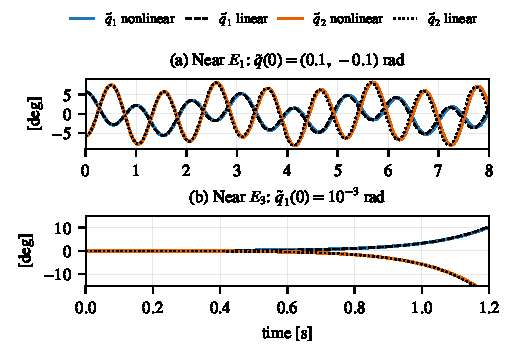
\includegraphics[width=\linewidth]{sim.pdf}
\captionof{figure}{Nonlinear (colour) vs.\ linear (black) responses near (a) $E_1$, (b) $E_3$.}\label{fig:sim}
\end{minipage}

% =====================================================================

% #####################################################################
%  PHASE 2
% #####################################################################
\clearpage
\phantomsection\label{phase2}
\begin{center}
\begin{singlespace}
{\fontsize{17}{20}\selectfont Phase 2: Stability Analysis of the Acrobot}\\[4pt]
{\small Bhargav (2025102061) \quad Sreekar (2025102074) \quad Kaushik (2025102071) \quad Divijat (2025102040)}\\[1pt]
{\footnotesize Control Systems Project \quad$\cdot$\quad Phase 2 Report \quad$\cdot$\quad November 5, 2026}
\end{singlespace}
\end{center}
\vspace{-6pt}
{\small\textbf{Abstract.} Using the Phase~1 model (Sections~I--V), we classify every equilibrium from the transfer functions and from $A$, link the result to the shape of $U$, and confirm it in a PyBullet simulation. At the upright $E_3$ we prove that static or PD feedback from one joint angle cannot stabilize it, and show that a dynamic observer-based controller can, for small offsets only.\par}

% =====================================================================
\begin{keep}
\section{Stability Criteria}
% =====================================================================
\subsection{Definitions}
For $\dot{\tilde x}=A\tilde x+B_\ell\tilde\tau$ and $G_j(s)=C_j(sI-A)^{-1}B_\ell=N_j(s)/\Delta(s)$, $C_j=e_j^T$:
\begin{equation}
\begin{aligned}
&\text{asymptotically stable} &&\Leftrightarrow\ \operatorname{Re}\lambda_i(A)<0\ \ \forall i, \qquad
&&\text{BIBO stable } (G_j) &&\Leftrightarrow\ \operatorname{Re}p<0\ \ \forall\text{ poles }p,\\
&\text{marginally stable} &&\Leftrightarrow\ \operatorname{Re}\lambda_i\le0,\ \text{simple on } j\mathbb R, \qquad
&&\text{nonlinear (Lyapunov indirect)} &&:\ \exists\operatorname{Re}\lambda_i>0\Rightarrow\text{unstable}.
\end{aligned}\label{eq:crit}
\end{equation}
\end{keep}
\begin{keep}
\subsection{Poles of $G_j$ = Eigenvalues of $A$}
At every equilibrium
\begin{equation*}
\operatorname{rank}\underbrace{[B_\ell\ \ AB_\ell\ \ A^2B_\ell\ \ A^3B_\ell]}_{\mathcal C}=4,\qquad
\operatorname{rank}\underbrace{[C_j;\ C_jA;\ C_jA^2;\ C_jA^3]}_{\mathcal O_j}=4\quad(j=1,2),
\end{equation*}
so each $G_j$ is a minimal realization (no pole--zero cancellation, Table~\ref{tab:tf}) and
$\{\text{poles of }G_1\}=\{\text{poles of }G_2\}=\{\lambda_i(A)\}$: \textbf{the transfer-function and state-space verdicts coincide}.
\end{keep}

\begin{keep}
\subsection{Characteristic Polynomial}
\begin{equation}
\Delta(s)=\det(sI-A)=s^4+\boxed{0}\,s^3-\operatorname{tr}(P)\,s^2+\boxed{0}\,s+\det P .\label{eq:delta}
\end{equation}
A Hurwitz polynomial has all coefficients $>0$; the $s^3$ and $s^1$ coefficients are $0$ (no friction) $\Rightarrow$ \textbf{no equilibrium is asymptotically stable for $\tau=0$}. With $\lambda=s^2=\operatorname{eig}(P)$:
\begin{equation}
\lambda^2-\operatorname{tr}(P)\,\lambda+\det P=0,\qquad
\lambda<0\Rightarrow s=\pm j\sqrt{-\lambda},\qquad \lambda>0\Rightarrow s=\pm\sqrt{\lambda}\ (\text{one RHP pole}).\label{eq:lam}
\end{equation}
\begin{center}
\captionof{table}{Pole pattern from the signs of $\det P$ and $\operatorname{tr}P$}\label{tab:cases}
\footnotesize\setlength{\tabcolsep}{8pt}\renewcommand{\arraystretch}{0.95}
\begin{tabular}{@{}ccccl@{}}
\toprule
$\det P$ & $\operatorname{tr}P$ & $\lambda_1,\lambda_2$ & poles & case\\
\midrule
$>0$ & $<0$ & both $<0$ & $\pm j\omega_1,\ \pm j\omega_2$ & $E_1$\\
$<0$ & any & opposite signs & $\pm\sigma,\ \pm j\omega$ & $E_2$, $E_4$\\
$>0$ & $>0$ & both $>0$ & $\pm\sigma_1,\ \pm\sigma_2$ & $E_3$\\
\bottomrule
\end{tabular}
\end{center}
\end{keep}

\begin{keep}
\subsection{Link to the Potential Energy}
\begin{equation}
K=\frac{\partial\tau_g}{\partial q}=-\nabla^2U,\qquad
P=M^{-1}K\ \sim\ M^{-1/2}KM^{-1/2}\ \ (M\succ0)
\;\overset{\text{Sylvester}}{\Longrightarrow}\;
\boxed{\#\{\text{RHP poles}\}=\#\{\text{negative eigenvalues of }\nabla^2U\}}\label{eq:inertia}
\end{equation}
Minimum of $U$ $\to$ 0 RHP poles, saddle $\to$ 1, maximum $\to$ 2 [3].

% =====================================================================
\end{keep}
\begin{keep}
\section{Stability of Each Equilibrium}
% =====================================================================
\begin{center}
\captionof{table}{Stability of the four equilibria (transfer functions, state matrix and energy agree)}\label{tab:stab}
\footnotesize\setlength{\tabcolsep}{4pt}\renewcommand{\arraystretch}{0.95}
\begin{tabular}{@{}ccccccl@{}}
\toprule
 & $(\operatorname{tr}P,\ \det P)$ & $\lambda=\operatorname{eig}P$ & poles of $G_1,G_2$ $=\operatorname{eig}A$ & $\operatorname{eig}\nabla^2U$ & RHP & verdict (linear\,/\,nonlinear)\\
\midrule
$E_1$ & $(-42.241,\ 186.772)$ & $-5.018,\ -37.224$ & $\pm j2.2400,\ \pm j6.1011$ & $4.905,\ 29.43$ (min) & 0 & marginal\,/\,Lyapunov stable\\
$E_2$ & $(-8.403,\ -186.772)$ & $-18.499,\ 10.096$ & $\pm3.1775,\ \pm j4.3010$ & $-14.715,\ 9.81$ (saddle) & 1 & unstable\,/\,unstable\\
$E_3$ & $(42.241,\ 186.772)$ & $5.018,\ 37.224$ & $\pm2.2400,\ \pm6.1011$ & $-29.43,\ -4.905$ (max) & 2 & unstable\,/\,unstable\\
$E_4$ & $(8.403,\ -186.772)$ & $-10.096,\ 18.499$ & $\pm4.3010,\ \pm j3.1775$ & $-9.81,\ 14.715$ (saddle) & 1 & unstable\,/\,unstable\\
\bottomrule
\end{tabular}
\end{center}
\end{keep}

\begin{keep}
\subsection{$E_1$ (down--down)}
\begin{itemize}
\item \textit{Transfer function:} simple poles on $j\mathbb R$ $\Rightarrow$ not BIBO stable. E.g.\ $\tau=\sin(2.24t)$: $\tilde Q_j(s)$ gets a double pole at $\pm j2.24$ $\Rightarrow$ $\tilde q_j\sim t\sin(2.24t)$.
\item \textit{State space:} $\tilde x(t)=\sum_{k=1}^{2}\big(a_k\cos\omega_kt+b_k\sin\omega_kt\big)v_k$, $\omega_{1,2}=2.24,\,6.10$ $\Rightarrow$ bounded, non-decaying: \textbf{marginally stable}.
\item \textit{Nonlinear (linearization inconclusive):} Lyapunov function [5]
\begin{equation}
V(x)=\tfrac12\dot q^TM(q)\dot q+U(q)-U(q^*),\qquad
\nabla^2U(q^*)\succ0\Rightarrow V\succ0\text{ near }E_1,\qquad
\dot V=\dot q^TB\tau=0 .\label{eq:lyap}
\end{equation}
$\Rightarrow$ \textbf{stable in the sense of Lyapunov, not asymptotically} ($V$ is constant: the swing never decays).
\end{itemize}
\end{keep}

\begin{keep}
\subsection{$E_2$, $E_4$ (one link up)}
$\det P=-186.772<0\Rightarrow\lambda_1\lambda_2<0$ $\Rightarrow$ one real pole in the RHP ($+3.1775$ at $E_2$, $+4.3010$ at $E_4$) $\Rightarrow$ BIBO unstable, $A$ unstable, nonlinear unstable by~\eqref{eq:crit}. $U$ has a saddle.
\end{keep}

\begin{keep}
\subsection{$E_3$ (up--up)}
$P_{E3}=-P_{E1}\Rightarrow\lambda(P_{E3})=-\lambda(P_{E1})=\{5.018,\,37.224\}\Rightarrow s=\pm2.2400,\ \pm6.1011$: \textbf{two RHP poles}, unstable in every sense. $U$ has a strict maximum.

% =====================================================================
\end{keep}
\begin{keep}
\section{Simulation Evidence}
% =====================================================================
\subsection{Simulator}
Nonlinear model in \textbf{PyBullet} [6] (uniform rods, no damping, step $h=0.25$~ms), run alongside the linear model~\eqref{eq:AB} from the same initial condition. Check against RK4 of~\eqref{eq:eom} with $q(0)=(0.8,-0.5)$~rad, $\tau=3\sin2t$:
$\max_{t\le5\,\text{s}}|q_{\text{PyBullet}}-q_{\text{RK4}}|=0.52^\circ$.
\end{keep}

\begin{figure}[H]
\centering
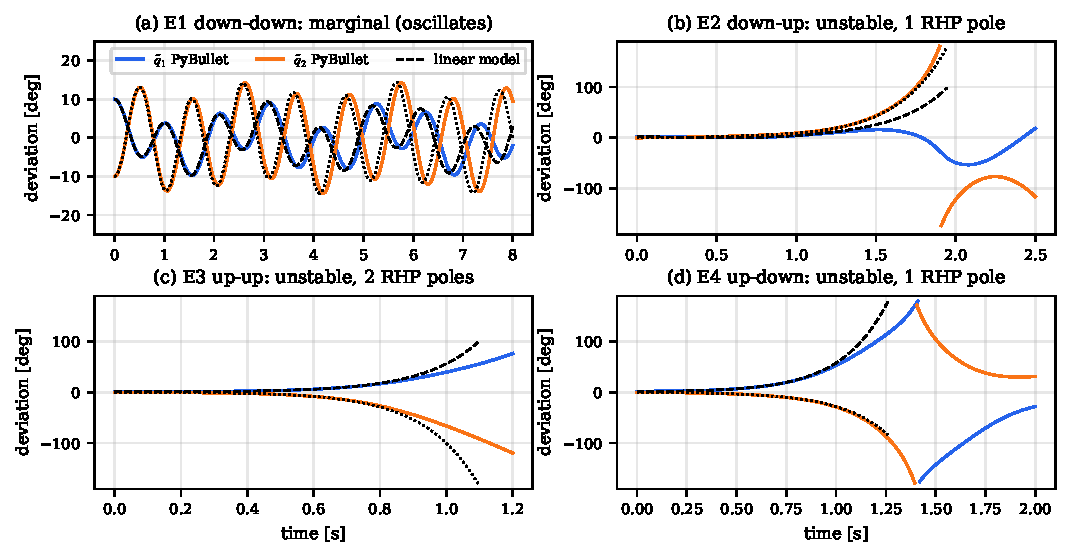
\includegraphics[width=0.9\textwidth]{fig_openloop.pdf}
\caption{Free response ($\tau=0$) near each equilibrium: PyBullet (colour) vs.\ linear model (black). Initial offsets: (a) $(10^\circ,-10^\circ)$; (b) $2^\circ$; (c) $1^\circ$; (d) $2^\circ$ on $q_1$.}\label{fig:ol}
\end{figure}

\begin{keep}
\subsection{Prediction vs.\ Measurement}
Near an unstable equilibrium $\|\tilde q(t)\|\approx c\,e^{p_{\max}t}$, so the measured rate is $\hat\sigma=\mathrm{d}\ln\|\tilde q\|/\mathrm{d}t$ (least-squares fit for $0.2^\circ<\|\tilde q\|<15^\circ$).
\begin{center}
\captionof{table}{Linear-model predictions vs.\ PyBullet measurements}\label{tab:evidence}
\footnotesize\setlength{\tabcolsep}{6pt}\renewcommand{\arraystretch}{0.95}
\begin{tabular}{@{}cllll@{}}
\toprule
 & quantity & predicted (linear) & measured (PyBullet) & error\\
\midrule
$E_1$ & oscillation frequencies (60~s run) & $2.240,\ 6.101$~rad/s & $2.239,\ 5.997$~rad/s & within 1 bin ($2\pi/60=0.105$)\\
$E_1$ & energy change over 60~s & $0$ & $1.2\times10^{-3}$~J & integration error\\
$E_2$ & growth rate $\hat\sigma$; time to $30^\circ$ from $0.05^\circ$ & $3.1775$~s$^{-1}$ & $3.171$~s$^{-1}$;\ $2.52$~s & $0.22\%$\\
$E_3$ & growth rate $\hat\sigma$; time to $30^\circ$ from $0.01^\circ$ & $6.1011$~s$^{-1}$ & $6.088$~s$^{-1}$;\ $1.55$~s & $0.21\%$\\
$E_4$ & growth rate $\hat\sigma$; time to $30^\circ$ from $0.05^\circ$ & $4.3010$~s$^{-1}$ & $4.294$~s$^{-1}$;\ $1.69$~s & $0.15\%$\\
\bottomrule
\end{tabular}
\end{center}
\end{keep}
\begin{figure}[H]
\centering
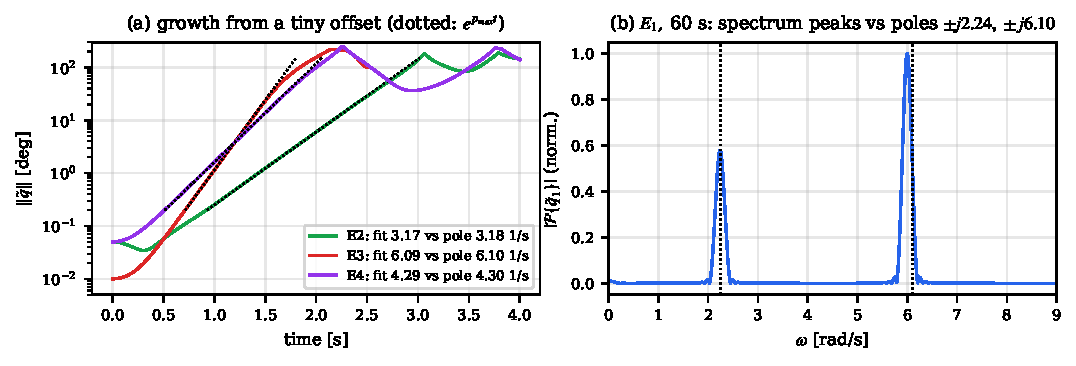
\includegraphics[width=0.9\textwidth]{fig_growth.pdf}
\caption{(a) $\|\tilde q\|$ from a tiny offset; dotted slope $=p_{\max}$. (b) Spectrum of $\tilde q_1$ near $E_1$; dotted lines are the poles.}\label{fig:growth}
\end{figure}

% =====================================================================
\begin{keep}
\section{Single-Angle Feedback at the Upright $E_3$}
% =====================================================================
\subsection{Loop}
Measure one angle, $y=\tilde q_j$, and apply $\tau=-C(s)\,y$ with $C=N_c/D_c$:
\begin{equation}
1+C(s)G_j(s)=0\ \Leftrightarrow\ \Delta(s)D_c(s)+N_j(s)N_c(s)=0 .\label{eq:loop}
\end{equation}
At $E_3$ (Table~\ref{tab:tf}), writing $\Delta=s^4+a_2s^2+a_0$ and $N_j=b_2s^2+b_0$:
\begin{center}
\captionof{table}{Plant data at $E_3$ ($a_2=-42.241$, $a_0=186.772$)}\label{tab:e3}
\footnotesize\setlength{\tabcolsep}{8pt}\renewcommand{\arraystretch}{0.95}
\begin{tabular}{@{}cccccc@{}}
\toprule
measured & $b_2$ & $b_0$ & $b_0/b_2$ & zeros $\pm z$ & RHP poles\\
\midrule
$q_1$ & $-3.0147$ & $12.6926$ & $-4.2103$ & $\pm2.0519$ & $2.2400,\ 6.1011$\\
$q_2$ & $6.0332$ & $-31.7316$ & $-5.2595$ & $\pm2.2934$ & $2.2400,\ 6.1011$\\
\bottomrule
\end{tabular}
\end{center}
\end{keep}

\begin{keep}
\subsection{Static and PD Feedback: Impossible}
With $C(s)=K_p+K_ds$, \eqref{eq:loop} becomes
\begin{equation}
s^4+(K_db_2)\,s^3+(a_2+K_pb_2)\,s^2+(K_db_0)\,s+(a_0+K_pb_0)=0 .\label{eq:pdpoly}
\end{equation}
\textit{Proof:} Hurwitz $\Rightarrow$ $K_db_2>0$ and $K_db_0>0$ $\Rightarrow$ $b_0/b_2>0$. But $b_0/b_2=-z^2<0$ for both angles (Table~\ref{tab:e3}) $\Rightarrow$ contradiction. \hfill$\blacksquare$
\begin{itemize}
\item $K_d=0$: \eqref{eq:pdpoly} is even, $p(s)=p(-s)$ $\Rightarrow$ roots symmetric about $j\mathbb R$ $\Rightarrow$ never Hurwitz.
\item Root locus: gain $\to0$, roots $\to\{\pm2.24,\pm6.10\}$; gain $\to\infty$, roots $\to\{-K_p/K_d,\ \pm z\}\ni+z$ $\Rightarrow$ a pole always remains in the RHP. The cause is the \textbf{real RHP zero} $+z$.
\item Grid $K_p\in[-400,400]$, $K_d\in[-150,150]$: $\min\max\operatorname{Re}\lambda=0.96$~s$^{-1}$ ($q_1$, at $K_p=-15$, $K_d=0$) and $2.29$~s$^{-1}$ ($q_2$, $\to z=2.2934$ at high gain). PyBullet with these gains: $1^\circ\to30^\circ$ in $1.0$~s ($q_1$) and $1.8$~s ($q_2$).
\end{itemize}
\end{keep}
\begin{figure}[H]
\centering
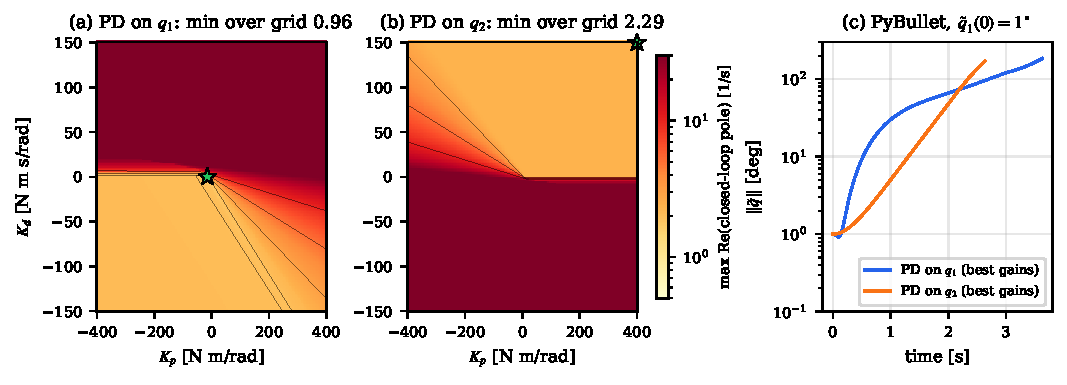
\includegraphics[width=0.93\textwidth]{fig_pd.pdf}
\caption{PD from one angle at $E_3$. (a, b) $\max\operatorname{Re}$ of the closed-loop poles over the gain plane: positive everywhere (star: best gains). (c) PyBullet with the best gains.}\label{fig:pd}
\end{figure}

\begin{keep}
\subsection{Dynamic Output Feedback: Possible but Fragile}
$\mathcal O_j$ has rank 4, so an observer reconstructs $\tilde x$ from $y=\tilde q_j$ alone:
\begin{equation}
\dot{\hat x}=A\hat x+B_\ell\tau+L\,(y-C_j\hat x),\qquad \tau=-K\hat x,\qquad
\lambda_{\text{cl}}=\lambda(A-B_\ell K)\ \cup\ \lambda(A-LC_j)\quad\text{(separation)}.\label{eq:obs}
\end{equation}
$K$ from LQR with $Q=\operatorname{diag}(10,10,1,1)$, $R=1$: $K=[-266.1,\,-107.4,\,-115.0,\,-54.3]$, $\lambda(A-B_\ell K)=\{-10.09,\,-4.25,\,-2.24\pm0.04j\}$. $L$ from the dual LQR problem. Two limits hold for \emph{any} controller:
\begin{equation}
\text{PIP [4]: stable } C(s)\text{ exists}\Leftrightarrow \#\{\text{real RHP poles in }(z,\infty)\}\text{ even};\qquad
\|S\|_\infty\ \ge\ \prod_i\frac{|z+p_i|}{|z-p_i|}\ \ [3].\label{eq:limits}
\end{equation}
$z$ sits just below the RHP pole $2.24$, so $|z-p_1|$ is small and $\|S\|_\infty$ is huge: the loop is very sensitive, and saturation at $20\Nm$ breaks it for offsets beyond the last column of Table~\ref{tab:obs}.
\begin{center}
\captionof{table}{Single-angle observer + LQR at $E_3$: design, fundamental limits and PyBullet results ($|\tau|\le20\Nm$)}\label{tab:obs}
\footnotesize\setlength{\tabcolsep}{4.5pt}\renewcommand{\arraystretch}{1.0}
\begin{tabular}{@{}cccccc@{}}
\toprule
measured & observer poles $\lambda(A-LC_j)$ & poles in $(z,\infty)$ & stable controller? & $\|S\|_\infty\ge$ & largest offset held: $\tilde q_1(0)$,\ $\tilde q_2(0)$\\
\midrule
$q_1$ & $-6.34,\,-5.88,\,-2.67,\,-1.90$ & $2.24,\ 6.10$ (even) & yes & $45.9$ & $1.42^\circ,\ 1.66^\circ$\\
$q_2$ & $-6.56,\,-5.67,\,-2.49,\,-2.03$ & $6.10$ (odd) & \textbf{no} (must be unstable) & $187$ & $0.23^\circ,\ 0.97^\circ$\\
full state & -- & -- & -- & -- & $4.64^\circ,\ 10.06^\circ$\\
\bottomrule
\end{tabular}
\end{center}
\end{keep}
\begin{figure}[H]
\centering
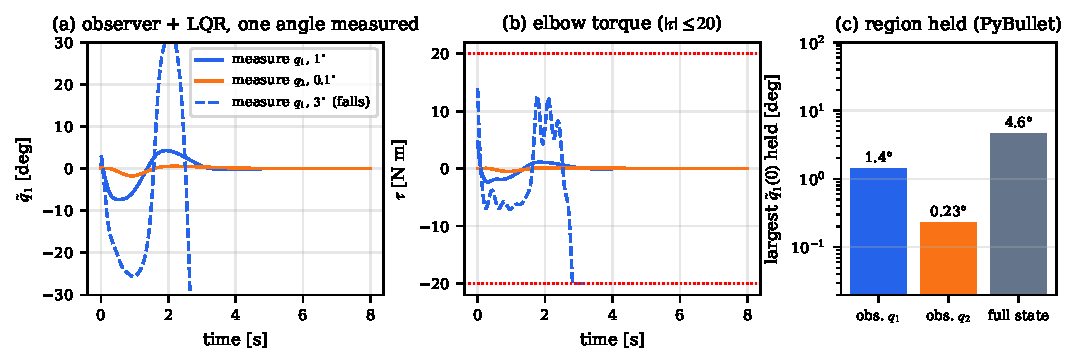
\includegraphics[width=0.9\textwidth]{fig_observer.pdf}
\caption{Observer + LQR at $E_3$ in PyBullet using one angle: (a) $\tilde q_1$; (b) torque; (c) largest initial offset still stabilized.}\label{fig:obs}
\end{figure}

\begin{keep}
\subsection{Answer}\mbox{}\par\smallskip
\noindent\fbox{\begin{minipage}{\dimexpr\linewidth-2\fboxsep-2\fboxrule}\sloppy
\begin{itemize}[leftmargin=1.2em]
\item \textbf{Static / PD feedback from one angle cannot stabilize $E_3$} (either angle): the real RHP zero gives $b_0/b_2<0$, which contradicts the Hurwitz conditions of~\eqref{eq:pdpoly}.
\item \textbf{A dynamic controller can}, since $(A,C_j)$ is observable for $j=1,2$. Via $q_1$ a stable controller suffices; via $q_2$ it must be unstable (PIP).
\item \textbf{It is fragile}: $\|S\|_\infty\ge46$ ($q_1$) or $187$ ($q_2$), and with $|\tau|\le20\Nm$ it holds only $\approx1.4^\circ$ ($q_1$) or $\approx0.2^\circ$ ($q_2$), vs.\ $4.6^\circ$ with full state. Full-state feedback is the route for Phase~3.
\end{itemize}
\end{minipage}}

% =====================================================================
\end{keep}
\begin{keep}
\section{Simulation Tools}
% =====================================================================
\begin{itemize}
\item \textbf{Interactive PyBullet simulator:} \texttt{phase2/acrobot\_phase2\_sim.py}, instructions in \texttt{phase2/README.md}. Live dashboard: choose equilibrium, initial condition (slider, typed value or drag), and controller (open loop, single-angle PD, single-angle observer + LQR); shows the nonlinear arm with the linear model, $\tilde q(t)$, $\tau(t)$ and the closed-loop poles.
\item \textbf{Reproducibility:} every figure and number above comes from \texttt{code/make\_phase2\_results.py} in the Phase~2 deliverable folder.
\item \textbf{Phase~2 animation} (Manim, 2K): \href{https://drive.google.com/file/d/19THfoXXzbdMtbteCKE4v0VRLpV869wE0/view?usp=sharing}{\textcolor{blue!60!black}{\textbf{watch the video}}}.
\end{itemize}
\end{keep}



% #####################################################################
%  PHASE 3
% #####################################################################
\clearpage
\phantomsection\label{phase3}
\begin{center}
\begin{singlespace}
{\fontsize{17}{20}\selectfont Phase 3: Control Around the Equilibria}\\[4pt]
{\small Bhargav (2025102061) \quad Sreekar (2025102074) \quad Kaushik (2025102071) \quad Divijat (2025102040)}\\[1pt]
{\footnotesize Control Systems Project \quad$\cdot$\quad Phase 3 Report \quad$\cdot$\quad November 5, 2026}
\end{singlespace}
\end{center}
\vspace{-6pt}
{\small\textbf{Abstract.} We stabilize all four equilibria: the upright $E_3$ and $E_2$, $E_4$ with full-state LQR, and $E_1$ with a PD controller on the elbow angle alone. Each choice is justified by a weight sweep or a Lyapunov argument. We then measure how far from each equilibrium the controller still recovers with $|\tau|\le20\Nm$, both analytically and with region-of-attraction maps of the nonlinear model.\par}

% =====================================================================
\begin{keep}
\section{Design Approach}
% =====================================================================
\subsection{Why Full-State Feedback}
Phase~2 showed that one measured angle is not enough at $E_3$: PD is impossible and an observer holds only $\approx1^\circ$. All four states are therefore fed back, which is possible because the system is controllable at every equilibrium ($\operatorname{rank}\mathcal C=4$, Sec.~VI-B). The motor is limited, so the applied torque is
\begin{equation}
\tau=\operatorname{sat}\!\big(-K\tilde x\big)=\max\!\big(-20,\ \min(20,\,-K\tilde x)\big),\qquad \tilde x=[\tilde q_1,\ \tilde q_2,\ \dot q_1,\ \dot q_2]^T .\label{eq:sat}
\end{equation}
\end{keep}

\begin{keep}
\subsection{LQR}
$K$ minimizes $J=\int_0^\infty\big(\tilde x^TQ\tilde x+R\,\tau^2\big)\,dt$ for the linear model~\eqref{eq:AB}:
\begin{equation}
A^TS+SA-SB_\ell R^{-1}B_\ell^TS+Q=0,\qquad K=R^{-1}B_\ell^TS .\label{eq:are}
\end{equation}
\begin{itemize}
\item \textit{Why LQR:} the closed loop is stable for any $Q\succeq0$, $R>0$ with $(A,B_\ell)$ controllable, and it keeps a phase margin $\ge60^\circ$ and gain margin $[\tfrac12,\infty)$ [7]. One scalar ($R$) trades speed against torque.
\item \textit{Weights:} $Q=I$ weighs $1$~rad of angle error like $1$~rad/s of rate error. $R$ is chosen by the sweep below.
\end{itemize}
\end{keep}

\begin{keep}
\subsection{Choice of $R$}
For each $R$ we compute $K$ and simulate the nonlinear saturated loop from a grid of initial offsets (Sec.~XIII-B). Fig.~\ref{fig:design}:
\begin{itemize}
\item $E_3$: the recovered area is almost flat ($16$--$20\%$ of a $\pm60^\circ$ grid for $10^{-3}\le R\le1$), while the fastest pole goes from $-10$ to $-214$~s$^{-1}$. The limit comes from $\tau_{\max}$, not from tuning. \textbf{$R=0.03$} is the knee: $93\%$ of the best area with a fastest pole of $-40$ instead of $-214$.
\item $E_2$: the region collapses for $R>0.3$ ($99\%\to90\%\to20\%$ at $R=0.3,\,0.56,\,1$) $\Rightarrow$ \textbf{$R=0.1$}. $E_4$: the area peaks at $R\approx0.1$--$0.18$ ($22$--$24\%$) and drops on both sides $\Rightarrow$ \textbf{$R=0.1$}.
\end{itemize}
\end{keep}
\begin{figure}[H]
\centering
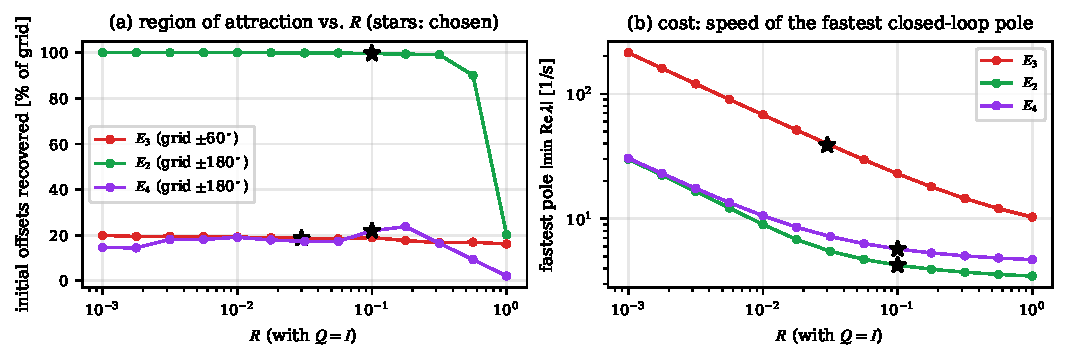
\includegraphics[width=0.9\textwidth]{fig_design.pdf}
\caption{Weight selection ($Q=I$). (a) Share of initial offsets recovered by the nonlinear saturated loop. (b) Fastest closed-loop pole, a measure of bandwidth and torque demand. Stars: chosen $R$.}\label{fig:design}
\end{figure}

\begin{keep}
\subsection{Comparison: Pole Placement at $E_3$}
Pole placement (\texttt{place}) at $\{-3,-4,-5,-6\}$ gives $K=[-322.9,\,-134.6,\,-138.1,\,-66.0]$. It settles faster for small offsets ($1.3$~s vs $4.1$~s from $2^\circ$) with less torque ($11.3$ vs $17.6\Nm$), but recovers a smaller region ($20\%$ vs $26\%$ of $\pm40^\circ$; $5^\circ$ vs $6^\circ$ along $q_1$). LQR is kept for $E_3$.
\end{keep}

\begin{keep}
\subsection{$E_1$: PD on the Elbow Angle Only}
At $E_1$ the zeros of $G_2$ are imaginary ($\pm j2.29$, Table~\ref{tab:tf}), so the sign conflict of~\eqref{eq:pdpoly} does not occur and a single angle suffices:
\begin{equation}
\tau=-K_p\tilde q_2-K_d\dot q_2,\qquad K_p=-5,\ K_d=0.4\quad\big(\text{best decay rate on a }(K_p,K_d)\text{ grid: }\max\operatorname{Re}\lambda=-0.52\big).\label{eq:e1pd}
\end{equation}
\textit{Proof of stability} (energy shaping, LaSalle [5]): with $E=T+U$, $\dot E=\dot q^TB\tau=\dot q_2\tau$, so
\begin{equation}
V_c=E-E^*+\tfrac12K_p\tilde q_2^{\,2},\qquad \dot V_c=-K_d\,\dot q_2^{\,2}\le0,\qquad
\nabla^2\!\big(U+\tfrac12K_p\tilde q_2^{\,2}\big)\big|_{E_1}:\ \lambda=0.760,\ 28.575>0 .\label{eq:vc}
\end{equation}
$V_c$ has a strict minimum at $E_1$ and never increases (while $|\tau|<20$), and $\dot q_2\equiv0$ forces $E_1$, so $E_1$ is asymptotically stable. Pure damping ($K_p=0$) also works but decays $19\times$ more slowly ($\max\operatorname{Re}\lambda=-0.027$): the slow mode swings both links together and barely moves the elbow.
\end{keep}

% =====================================================================
\begin{keep}
\section{Controllers}
% =====================================================================
\begin{center}
\captionof{table}{Phase 3 controllers ($\tau=\operatorname{sat}(-K\tilde x)$) and their linearized closed-loop poles}\label{tab:ctrl}
\footnotesize\setlength{\tabcolsep}{5pt}\renewcommand{\arraystretch}{1.0}
\begin{tabular}{@{}llll@{}}
\toprule
controller & design & $K=[k_{q_1},\ k_{q_2},\ k_{\dot q_1},\ k_{\dot q_2}]$ & closed-loop poles\\
\midrule
$E_3$ LQR & $Q=I$, $R=0.03$ & $[-503.0,\ -203.9,\ -218.3,\ -101.5]$ & $-39.86,\ -2.25\pm0.10j,\ -1.34$\\
$E_3$ pole placement & $\{-3,-4,-5,-6\}$ & $[-322.9,\ -134.6,\ -138.1,\ -66.0]$ & $-6,\ -5,\ -4,\ -3$\\
$E_2$ LQR & $Q=I$, $R=0.1$ & $[6.60,\ 46.49,\ 5.23,\ 13.24]$ & $-4.26,\ -2.40,\ -1.24\pm4.16j$\\
$E_4$ LQR & $Q=I$, $R=0.1$ & $[-49.31,\ 38.91,\ -13.19,\ 6.10]$ & $-5.73,\ -3.21,\ -0.96\pm3.08j$\\
$E_1$ elbow PD & $K_p=-5$, $K_d=0.4$ & $[0,\ -5,\ 0,\ 0.4]$ & $-0.69\pm2.31j,\ -0.52\pm2.14j$\\
\bottomrule
\end{tabular}
\end{center}
All poles are in the LHP, so every controller stabilizes its equilibrium locally. The $E_3$ gains are about $10\times$ larger than at $E_2$/$E_4$: the upright has two RHP poles, up to $+6.10$.
\end{keep}

% =====================================================================
\begin{keep}
\section{Limits with $\tau_{\max}=20\Nm$}
% =====================================================================
\subsection{Guaranteed Region (Analytic)}
Inside the level set $\Omega_c=\{\tilde x^TS\tilde x\le c\}$ the command never saturates when
\begin{equation}
\max_{\tilde x\in\Omega_c}|K\tilde x|=\sqrt{c\,KS^{-1}K^T}\le\tau_{\max}\ \Rightarrow\
c^*=\frac{\tau_{\max}^2}{KS^{-1}K^T},\qquad \dot V=-\tilde x^T\big(Q+K^TRK\big)\tilde x<0\ \text{ on }\Omega_{c^*} .\label{eq:ellipse}
\end{equation}
So the linear loop started in $\Omega_{c^*}$ stays unsaturated and converges. At rest ($\dot q=0$) this guarantees $|\tilde q_1|\le\sqrt{c^*/S_{11}}$ or $|\tilde q_2|\le\sqrt{c^*/S_{22}}$: $0.72^\circ/1.66^\circ$ ($E_3$), $45.6^\circ/19.9^\circ$ ($E_2$), $20.0^\circ/23.1^\circ$ ($E_4$). The bound is conservative because the loop usually survives short saturation.
\end{keep}

\begin{keep}
\subsection{Simulated Region of Attraction}
The real limits come from simulating the nonlinear saturated loop~\eqref{eq:sat} from a grid of offsets $(\tilde q_1(0),\tilde q_2(0))$ at rest. A start counts as recovered if after 10~s (30~s for $E_1$) $|\tilde q_i|<1^\circ$ and $|\dot q_i|<0.05$~rad/s, modulo $2\pi$. The grids are $81\times81$ ($\pm40^\circ$) at $E_3$ and $73\times73$ ($\pm180^\circ$) elsewhere. They use an RK4 integration ($h=2$~ms) of~\eqref{eq:eom}, which matches PyBullet on $100\%$ of 45 random grid points and $96\%$ of 45 points on the boundary. The region is not one solid piece: beyond its main part there are thin stripes of starts that swing away and are caught again. The axis limits quoted below are therefore the unbroken range out from $q^*$.
\end{keep}
\begin{figure}[H]
\centering
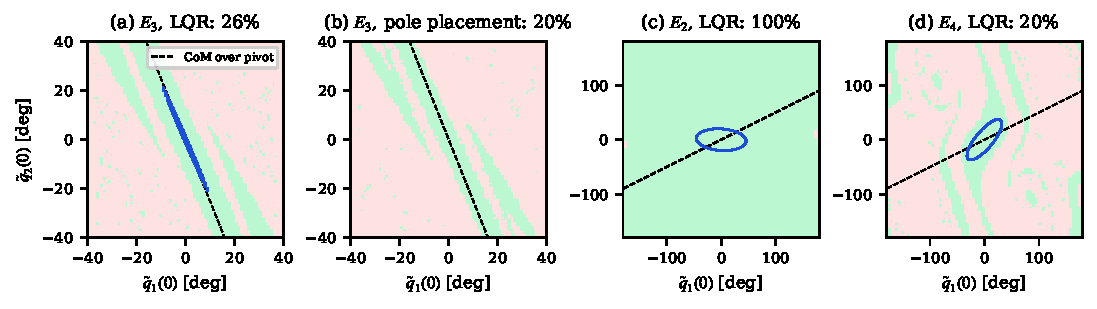
\includegraphics[width=0.97\textwidth]{fig_roa.pdf}
\caption{Region of attraction (green: recovered) with $|\tau|\le20\Nm$, starting at rest. Blue ellipse: guaranteed region~\eqref{eq:ellipse}. Dashed: offsets with the centre of mass over the pivot.}\label{fig:roa}
\end{figure}

\begin{keep}
\begin{center}
\captionof{table}{How far from the equilibrium each controller still works ($|\tau|\le20\Nm$, nonlinear model)}\label{tab:limits}
\footnotesize\setlength{\tabcolsep}{3.5pt}\renewcommand{\arraystretch}{1.0}
\begin{tabular}{@{}lcccccccc@{}}
\toprule
controller & recovered & $|\tilde q_1(0)|$ & $|\tilde q_2(0)|$ & along CoM line & guaranteed & shoulder kick & settling & peak $|\tau|$\\
 & (grid) & alone & alone & & $\tilde q_1$ / $\tilde q_2$ & $|\dot q_1(0)|$ & (2\%) & \\
\midrule
$E_3$ LQR & $26\%$ ($\pm40^\circ$) & $6^\circ$ & $13^\circ$ & $\ge43^\circ$ (grid edge) & $0.72^\circ$ / $1.66^\circ$ & $0.20$~rad/s & $4.1$~s ($2^\circ$) & $17.6$ ($2^\circ$)\\
$E_3$ pole pl. & $20\%$ ($\pm40^\circ$) & $5^\circ$ & $9^\circ$ & $\ge43^\circ$ (grid edge) & -- & $0.15$~rad/s & $1.3$~s ($2^\circ$) & $11.3$ ($2^\circ$)\\
$E_2$ LQR & $99.7\%$ ($\pm180^\circ$) & $175^\circ$ & $180^\circ$ & full grid & $45.6^\circ$ / $19.9^\circ$ & $\ge8$~rad/s & $3.0$~s & $20$ (sat.\ $3\%$)\\
$E_4$ LQR & $20.5\%$ ($\pm180^\circ$) & $35^\circ$ & $55^\circ$ & $47^\circ$ & $20.0^\circ$ / $23.1^\circ$ & $2.1$~rad/s & $3.6$~s & $4.5$\\
$E_1$ elbow PD & $77.8\%$ ($\pm180^\circ$) & $40^\circ$ & $115^\circ$ & $109^\circ$ & -- & $2.15$~rad/s & $12.8$~s & $5.3$\\
\bottomrule
\end{tabular}
\end{center}
{\footnotesize Settling and peak torque: $E_3$ from $\tilde q_1(0)=2^\circ$; $E_2$ from $(60^\circ,90^\circ)$; $E_4$ from $(20^\circ,30^\circ)$; $E_1$ from $(60^\circ,-60^\circ)$ (PyBullet).\par}
\end{keep}

\begin{keep}
\subsection{Why the Upright Region Is a Thin Band}
Linearizing $\tau_g$ at $E_3$ ($K_{E3}=-K_{E1}$, Table~\ref{tab:lin}):
\begin{equation}
\tau_{g,1}=9.81\,\big(2.5\,\tilde q_1+\tilde q_2\big),\qquad \tau_{g,2}=9.81\,\big(\tilde q_1+\tilde q_2\big).\label{eq:tg3}
\end{equation}
Gravity pushes the \emph{passive} shoulder with a torque $\propto 2.5\tilde q_1+\tilde q_2$, the horizontal offset of the total centre of mass. The motor cannot act on the shoulder directly; it must cancel this torque through the coupling $M_{12}$, which costs elbow torque. Along $\tilde q_2=-2.5\,\tilde q_1$ (CoM over the pivot) there is no shoulder torque, and the region stretches to the grid edge. Across that line every degree of CoM offset costs torque, so $20\Nm$ is used up after $6^\circ$ in $q_1$: the $2^\circ$ response already peaks at $17.6\Nm$. A shoulder kick of only $0.2$~rad/s is enough to break it.
\end{keep}

% =====================================================================
\begin{keep}
\section{Time Responses (PyBullet)}
% =====================================================================
\begin{itemize}
\item $E_3$ LQR (Fig.~\ref{fig:e3}): held from $\tilde q_1(0)=5.5^\circ$ (torque briefly saturated, $0.13$~s in total), falls from $7.5^\circ$ (bang--bang torque, arm swings away). Held from $(-10^\circ,25^\circ)$, a large but CoM-balanced offset, with peak torque only $3.3\Nm$.
\item $E_2$, $E_4$, $E_1$ (Fig.~\ref{fig:others}): each converges from a large offset. For $E_1$, $V_c$ in~\eqref{eq:vc} decreases monotonically, as the proof requires.
\end{itemize}
\end{keep}
\begin{figure}[H]
\centering
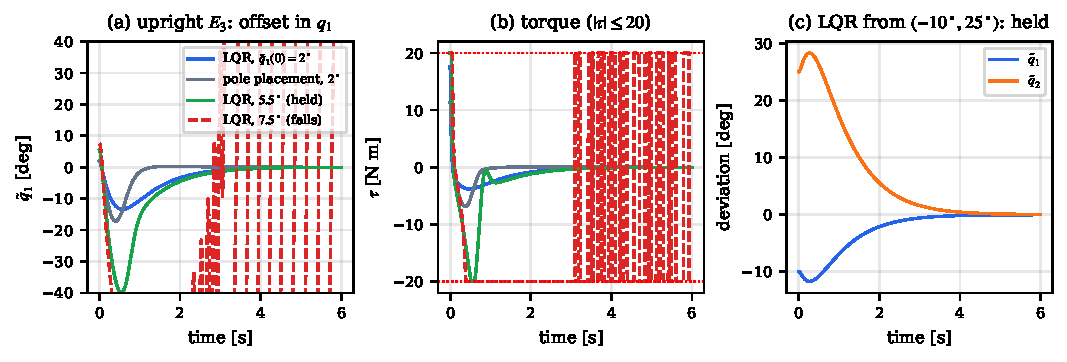
\includegraphics[width=0.9\textwidth]{fig_e3.pdf}
\caption{Upright $E_3$ in PyBullet. (a) $\tilde q_1$ for LQR and pole placement from several offsets in $q_1$; (b) torque; (c) a CoM-balanced offset.}\label{fig:e3}
\end{figure}
\begin{figure}[H]
\centering
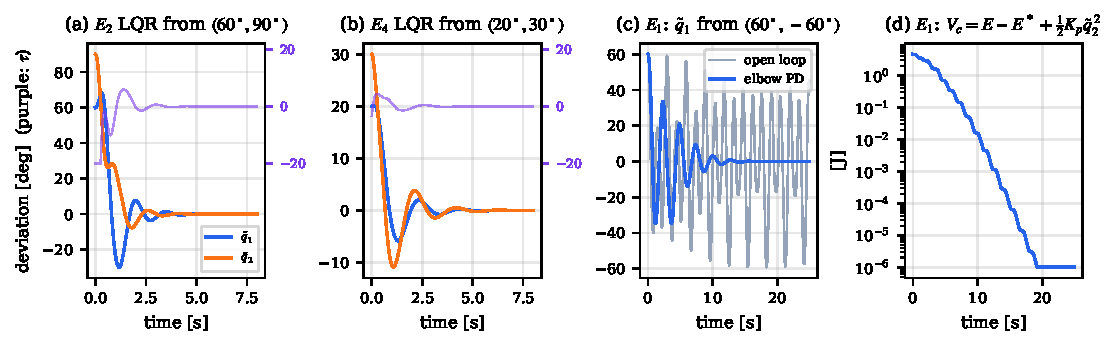
\includegraphics[width=0.95\textwidth]{fig_others.pdf}
\caption{(a) $E_2$ and (b) $E_4$ with LQR (purple: torque); (c) $E_1$ with elbow PD vs.\ open loop; (d) $V_c$ of~\eqref{eq:vc} along the $E_1$ run.}\label{fig:others}
\end{figure}

\begin{keep}
\subsection{Answer}\mbox{}\par\smallskip
\noindent\fbox{\begin{minipage}{\dimexpr\linewidth-2\fboxsep-2\fboxrule}\sloppy
\begin{itemize}[leftmargin=1.2em]
\item \textbf{Upright $E_3$:} full-state LQR ($Q=I$, $R=0.03$). It recovers from $6^\circ$ in $q_1$ or $13^\circ$ in $q_2$, and from $\ge43^\circ$ along the CoM-over-pivot line; $0.72^\circ$ is guaranteed analytically. The limit is $\tau_{\max}$, not the weights.
\item \textbf{$E_2$:} LQR ($R=0.1$) recovers from almost any rest position ($99.7\%$ of $\pm180^\circ$). \textbf{$E_4$:} LQR ($R=0.1$), $35^\circ$/$55^\circ$ along each axis.
\item \textbf{$E_1$:} PD on the elbow angle alone, proven asymptotically stable by energy shaping; $78\%$ of $\pm180^\circ$ recovered.
\end{itemize}
\end{minipage}}
\end{keep}

% =====================================================================
\begin{keep}
\section{Simulation and Code (Phase 3)}
% =====================================================================
\begin{itemize}
\item \textbf{Interactive simulator:} \texttt{phase3/acrobot\_phase3\_sim.py}, instructions in \texttt{phase3/README.md}. It is the Phase~2 dashboard plus the Phase~3 controllers (full-state LQR, pole placement, elbow PD).
\item \textbf{MATLAB:} \texttt{code/matlab/Acrobot\_Phase3\_Main.m} designs every controller (\texttt{lqr}, \texttt{place}), prints Tables~\ref{tab:ctrl} and the guaranteed regions, runs the nonlinear loops with \texttt{ode45} and maps the regions of attraction. Its results match the Python ones.
\item \textbf{Reproducibility:} every figure and number in Phase~3 comes from \texttt{code/make\_phase3\_results.py}.
\item \textbf{Phase~3 animation} (Manim, 2K): \href{https://drive.google.com/file/d/1c-7Yy664ZP4TCJIeDbrAmFozHC8frao1/view?usp=sharing}{\textcolor{blue!60!black}{\textbf{watch the video}}}.
\end{itemize}
\end{keep}

\begin{keep}
\vspace{6pt}
\begin{singlespace}
{\footnotesize
\textbf{References.}
[1] M.~W. Spong, ``The swing up control problem for the Acrobot,'' \emph{IEEE Control Syst. Mag.}, vol.~15, no.~1, pp.~49--55, 1995.\quad
[2] R.~Tedrake, \emph{Underactuated Robotics}, MIT, 2024. [Online]. Available: https://underactuated.csail.mit.edu\quad
[3] S.~Skogestad and I.~Postlethwaite, \emph{Multivariable Feedback Control}, 2nd ed., Wiley, 2005.\quad
[4] D.~C. Youla, J.~J. Bongiorno and C.~N. Lu, ``Single-loop feedback-stabilization of linear multivariable dynamical plants,'' \emph{Automatica}, vol.~10, pp.~159--173, 1974.\quad
[5] H.~K. Khalil, \emph{Nonlinear Systems}, 3rd ed., Prentice Hall, 2002.\quad
[6] E.~Coumans and Y.~Bai, ``PyBullet, a Python module for physics simulation,'' 2016--2024. [Online]. Available: https://pybullet.org\quad
[7] B.~D.~O. Anderson and J.~B. Moore, \emph{Optimal Control: Linear Quadratic Methods}, Prentice Hall, 1990.\par}
\end{singlespace}
\end{keep}

\end{document}
